%\documentclass[honours,12pt,twoside]{unswthesis}

\usepackage{afterpage}
\usepackage{amsfonts}
\usepackage{amsmath}
\usepackage{amssymb}
\usepackage{amsthm}
\usepackage[english]{babel}
\usepackage{graphicx}
\usepackage{natbib}
\usepackage[utf8]{inputenc}
\usepackage{latexsym}
\usepackage{url}
\usepackage{todonotes}
\usepackage{tikz}
\usepackage{pdfpages}
\usetikzlibrary{arrows}
\usepackage{float}

\usepackage{booktabs}
\renewcommand{\arraystretch}{1.2}


%%%%%%%%%%%%%%%%%%%%%%%%%%%%%%%%%%%%%%%%%%%%%%%%%%%%%%%%%%%%%%%%%
%
%  The following are some simple LaTeX macros to give some
%  commonly used letters in funny fonts. You may need more or less of
%  these
%
\newcommand{\R}{\mathbb{R}}
\newcommand{\Q}{\mathbb{Q}}
\newcommand{\C}{\mathbb{C}}
\newcommand{\N}{\mathbb{N}}
\newcommand{\F}{\mathbb{F}}
\newcommand{\PP}{\mathbb{P}}
\newcommand{\T}{\mathbb{T}}
\newcommand{\Z}{\mathbb{Z}}
\newcommand{\B}{\mathfrak{B}}
\newcommand{\BB}{\mathcal{B}}
\newcommand{\M}{\mathfrak{M}}
\newcommand{\X}{\mathfrak{X}}
\newcommand{\Y}{\mathfrak{Y}}
\newcommand{\CC}{\mathcal{C}}
\newcommand{\E}{\mathbb{E}}
\newcommand{\cP}{\mathcal{P}}
\newcommand{\cS}{\mathcal{S}}
\newcommand{\A}{\mathcal{A}}
\newcommand{\ZZ}{\mathcal{Z}}

%%%%%%%%%%%%%%%%%%%%%%%%%%%%%%%%%%%%%%%%%%%%%%%%%%%%%%%%%%%%%%%%%%%%%
%
% The following are much more esoteric commands that I have left in
% so that this file still processes. Use or delete as you see fit
%
\newcommand{\bv}[1]{\mbox{BV($#1$)}}
\newcommand{\comb}[2]{\left(\!\!\!\begin{array}{c}#1\\#2\end{array}\!\!\!\right)
}
\newcommand{\Lat}{{\rm Lat}}
\newcommand{\var}{\mathop{\rm var}}
\newcommand{\Pt}{{\mathcal P}}
\def\tr(#1){{\rm trace}(#1)}
\def\Exp(#1){{\mathbb E}(#1)}
\def\Exps(#1){{\mathbb E}\sparen(#1)}
\newcommand{\floor}[1]{\left\lfloor #1 \right\rfloor}
\newcommand{\ceil}[1]{\left\lceil #1 \right\rceil}
\newcommand{\hatt}[1]{\widehat #1}
\newcommand{\modeq}[3]{#1 \equiv #2 \,(\text{mod}\, #3)}
\newcommand{\rmod}{\,\mathrm{mod}\,}
\newcommand{\p}{\hphantom{+}}
\newcommand{\vect}[1]{\mbox{\boldmath $ #1 $}}
\newcommand{\reff}[2]{\ref{#1}.\ref{#2}}
\newcommand{\psum}[2]{\sum_{#1}^{#2}\!\!\!'\,\,}
\newcommand{\bin}[2]{\left( \begin{array}{@{}c@{}}
				#1 \\ #2
			\end{array}\right)	}
%
%  Macros - some of these are in plain TeX (gasp!)
%
\newcommand{\be}{($\beta$)}
\newcommand{\eqp}{\mathrel{{=}_p}}
\newcommand{\ltp}{\mathrel{{\prec}_p}}
\newcommand{\lep}{\mathrel{{\preceq}_p}}
\def\brack#1{\left \{ #1 \right \}}
\def\bul{$\bullet$\ }
\def\cl{{\rm cl}}
\let\del=\partial
\def\enditem{\par\smallskip\noindent}
\def\implies{\Rightarrow}
\def\inpr#1,#2{\t \hbox{\langle #1 , #2 \rangle} \t}
\def\ip<#1,#2>{\langle #1,#2 \rangle}
\def\lp{\ell^p}
\def\maxb#1{\max \brack{#1}}
\def\minb#1{\min \brack{#1}}
\def\mod#1{\left \vert #1 \right \vert}
\def\norm#1{\left \Vert #1 \right \Vert}
\def\paren(#1){\left( #1 \right)}
\def\qed{\hfill \hbox{$\Box$} \smallskip}
\def\sbrack#1{\Bigl \{ #1 \Bigr \} }
\def\ssbrack#1{ \{ #1 \} }
\def\smod#1{\Bigl \vert #1 \Bigr \vert}
\def\smmod#1{\bigl \vert #1 \bigr \vert}
\def\ssmod#1{\vert #1 \vert}
\def\sspmod#1{\vert\, #1 \, \vert}
\def\snorm#1{\Bigl \Vert #1 \Bigr \Vert}
\def\ssnorm#1{\Vert #1 \Vert}
\def\sparen(#1){\Bigl ( #1 \Bigr )}

\newcommand\blankpage{%
    \null
    \thispagestyle{empty}%
    \addtocounter{page}{-1}%
    \newpage}
    
%%%%%%%%%%%%%%%%%%%%%%%%%%%%%%%%%%%%%%%%%%%%%%%%%%%%%%%%%%%%%%
%
% These environments allow you to get nice numbered headings
%  for your Theorems, Definitions etc.  
%
%  Environments
%
%%%%%%%%%%%%%%%%%%%%%%%%%%%%%%%

\newtheorem{theorem}{Theorem}[section]
\newtheorem{lemma}[theorem]{Lemma}
\newtheorem{proposition}[theorem]{Proposition}
\newtheorem{corollary}[theorem]{Corollary}
\newtheorem{conjecture}[theorem]{Conjecture}
\newtheorem{definition}[theorem]{Definition}
\newtheorem{example}{Example}
\newtheorem{remark}[theorem]{Remark}
\newtheorem{question}[theorem]{Question}
\newtheorem{notation}[theorem]{Notation}
\numberwithin{equation}{section}

%\begin{document}

\chapter{Existing methodologies}\label{litrev}

This chapter outlines existing models in more detail, and discusses the impact of including location-based variables. In particular, we examine the variable thresholds developed by Yokoyama et al. \cite{Yokoyama2007} and the location-based \textsc{cnn} by Ghafoorian et al. \cite{GhafoorianM.2017Dml3}.

\section{Thresholding}\label{litrev-threshold}

This section describes an existing attempt to automate the identification of lacunes by developing and applying thresholds for certain variables. In 2007, Yokoyama et al. \cite{Yokoyama2007} developed an algorithm that identifies lacune candidates by examining their \textit{area}, \textit{circularity} and \textit{gravitational centre}. Area $A$ is the number of pixels that the candidate lacune covers. Circularity is given by $C = 4\pi\times\dfrac{A}{\ell^2}$, where $\ell$ is the perimeter of the candidate lacune. The gravitational centre is given by $(g_x, g_y) = \bigg(\dfrac{1}{n}\sum_{i=1}^nx_i, \dfrac{1}{n}\sum_{i=1}^ny_i\bigg)$.

Yokoyama et al. \cite{Yokoyama2007} claim that lacunes primarily occur in the basal ganglia, a structure at the centre of the brain. Thus the search for lacunes was limited to a central circular region with the coordinates of the centre and the radius specified for each scan.

Candidate lacunes satisfy thresholds based on area, circularity and gravitational centre. The thresholds are established dependent on the intensity of the surrounding structures. For this reason, candidates are separated into two categories: isolated lacunes and those surrounded by \textsc{wmh}. Isolated lacune candidates are determined by extracting the cerebral ventricle and calculating the mean pixel intensity. Candidates are determined as regions with an intensity below 70\% of the mean value. Isolated candidate lacunes satisfy the inequalities
\begin{align*}
	& 19 \le A \le 200, \\
	& 0.45 \le C,\text{ and } \\
	& (g_x - c_x)^2 + (g_y - c_y)^2 < 12000,
\end{align*}
where $(c_x, c_y)$ is the centre of the circular region of interest. The region defining accepted candidates is shown in Figure \ref{litrev-area-circ}.

% Fig. 5 from Yokoyama 2007 showing the bounds for area and circularity for false and true lacunes.
\begin{figure}[ht]
\centering
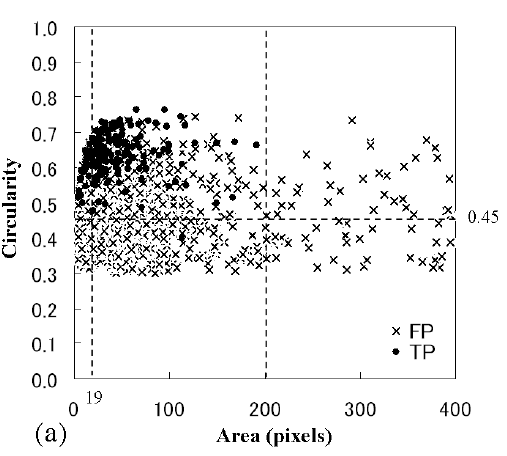
\includegraphics[scale=0.7]{Images/5_yokoyama_reg.png}
\caption{Relationship between candidate lacune area and circularity on the training data set.}
\small Image taken from \cite{Yokoyama2007}
\label{litrev-area-circ}
\end{figure}

Lacunes that appear next to \textsc{wmh} are more difficult to extract and so are treated separately. These candidates are determined by taking intensity differences between the region and the cerebral ventricle \textsc{csf}. Candidates satisfy the inequalities,
\begin{align*}
	25 \le A \le 100\text{ and } 0.48 \le C.
\end{align*}

Once candidates are identified, the model eliminates false-positives by examining the T1-weighted scans. False-positive removal is based on a candidate's location, area and gravitational centre.

The data set used to develop the model consisted of 100 scans, totalling 832 axial slices. Model training and testing consisted of 20 and 80 scans respectively. The final algorithm exhibited a \textit{sensitivity} rate (correct classification of positives) of 90.1\% and averaged 1.7 false-positives per slice.

Although the testing sensitivity was high, it was insufficient for the model to be usable on its own. Model improvement is required before it can be used to aid clinicians reliably. The low sensitivity rate may be the result of a restricted search area. Yokoyama et al. \cite{Yokoyama2007} made the assumption that lacunes only occur deep within the brain, through the basal ganglia. This was the motivation behind defining a circular search region and extracting the cerebral ventricles. However, this assumption is not always satisfied. Though less common, lacunes have been found in other brain regions, including the cerebrum (see Section \ref{data}). Restricting the search area may inadvertently exclude lacunes from detection.

The model by Yokoyama was dependent on a number of existing architectures. The first is the identification and extraction of particular brain regions. In this model, Yokoyama et al. were able to use existing binarisation techniques to extract the cerebral ventricle. Each sample also requires a calculated area, circularity and gravitational centre. Each of these calculations requires sufficient time and resources particularly if these calculations are to be conducted manually.

The comparatively low sensitivity may also be the result of too few variables. An indicator for hyperintensive rims and the area and circularity from associated \textsc{flair} images may improve the sensitivity rate. This was not tested due to time and data constraints.

%
%
%This section describes an existing attempt to automate the identification of lacunes, with false-positives reduced by accepting candidates within established thresholds for certain variables. In 2007, Yokoyama et al. \cite{Yokoyama2007} developed an algorithm that examines lacune candidate area, circularity and gravitational centre. Candidates are chosen such that they satisfy particular thresholds, where these thresholds are dependent on the candidate's location and surrounding hyperintense structures. The resulting model exhibited a \textit{sensitivity} rate (correct classification of positives) of 90.1\% and averaged 1.7 false-positives per axial slice.
%
%% Fig 1. from Yokoyama 2007 that shows structure of algorithm
%\begin{figure}[ht]
%\centering
%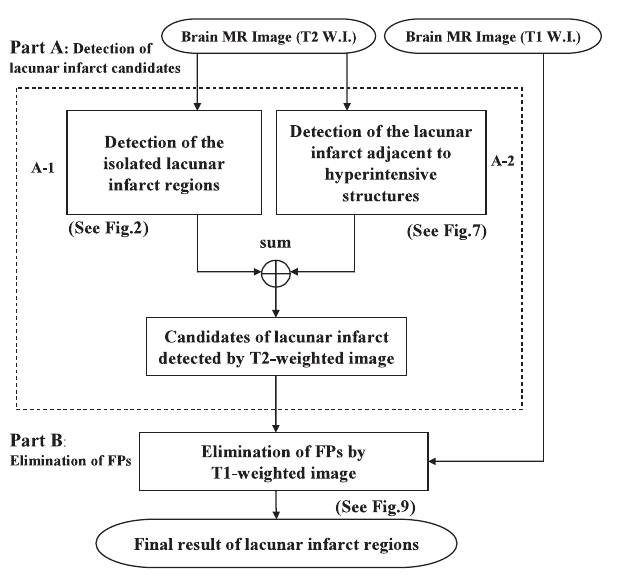
\includegraphics[scale=0.7]{Images/5_yokoyama_model.png}
%\caption{Model structure by Yokoyama et al. \citep{Yokoyama2007}}
%\label{litrev-yokoyama-structure}
%\end{figure}
%
%The algorithm is comprised of several stages, shown in Figure \ref{litrev-yokoyama-structure}. In the first phase, T2-weighted images are used to identify candidate lacunes. These candidates are one of two types: lacunes that are isolated, and those that are found next to \textsc{wmh}.
%
%% Fig. 3 from Yokoyama 2007
%\begin{figure}[ht]
%	\centering
%	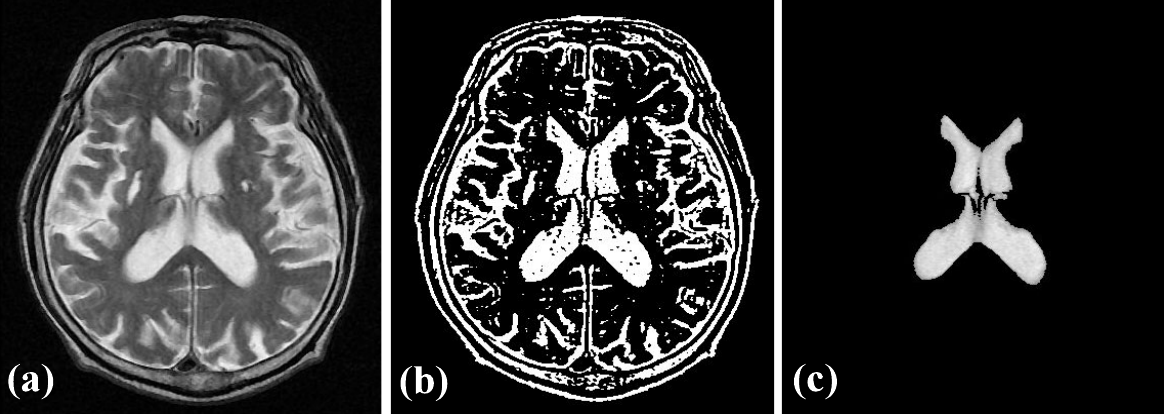
\includegraphics[width=\textwidth]{Images/5_extract_ventricle.png}
%	\caption{Extraction of the cerebral ventricle.}
%	\small Image taken from \cite{Yokoyama2007}
%	\label{litrev-yokoyama-ventricles}
%\end{figure}
%
%Isolated lacune candidates are determined by considering the mean pixel value of the cerebral ventricles. The ventricles are extracted from the image, shown in Figure \ref{litrev-yokoyama-ventricles}, and the threshold for lacune identification is set at 70\% of the mean pixel value. Yokoyama et al. \cite{Yokoyama2007} claim that lacunes primarily occur in the basal ganglia, a structure at the centre of the brain. Hence, the detection region is limited to a central circular region with determined centre and radius for each scan. 
%
%Lacunes are identified by considering three properties: area, circularity and gravitational centre. \textit{Area}, $A$, is the number of pixels that the candidate lacune covers. \textit{Circularity}, $C$, is given by $	C = 4\pi \times \dfrac{A}{\ell^2}$, where $\ell$ is the perimeter of the candidate lacune. The \textit{gravitational centre} is the central coordinate of the candidate lacune, given by $(g_x, g_y) = \bigg(\dfrac{1}{n}\sum_{i=1}^nx_i, \dfrac{1}{n}\sum_{i=1}^ny_i\bigg)$. Candidate lacunes satisfy the inequalities
%\begin{align*}
%	& 19 \le A \le 200, \\
%	& 0.45 \le C,\text{ and } \\
%	& (g_x - c_x)^2 + (g_y - c_y)^2 < 12000,
%\end{align*}
%where $(c_x, c_y)$ is the centre of the circular region of interest. The candidate regions for area and circularity are shown in Figure \ref{litrev-area-circ}.
%


%Lacunes that appear next to \textsc{wmh} are more difficult to extract and so are treated separately. Yokoyama et al. use the difference between two circular filters of radii 1 and 8 pixels. False-positives are eliminated by taking the difference in intensity between candidate lacunes and cerebral ventricle \textsc{csf}. Using the same definitions for area and circularity as with isolated lacunes, candidates next to \textsc{wmh} satisfy
%\[
%	25 \le A \le 100\text{ and } 0.48 \le C.
%\]
%Once candidates are identified, the model eliminates false-positives by examining the T1-weighted scans. False-positive removal is based on candidate location, area and gravitational centre.
%
%The algorithm was trained on 100 scans, containing 832 slices in total. 20 of these scans were used for training and 80 for testing.
%
%The second phase of training reduced the number of false-positives by 68\%. However, of the four types of false-positives, enlarged perivascular spaces had no reduction, as shown in Figure \ref{litrev-yokoyama-fps}. Other false-positives types include those at the edge of the cerebral parenchyma (\textsc{ecp}), periventricular high-signal regions (\textsc{pvh}), and those around the cerebral ventricle (\textsc{cv}), and will not be discussed. This model is instead more likely to differentiate lacunes from the edge of the cerebrum, hyperintensities and the cerebral ventricle.
%
%% Table 1 from Yokoyama 2007. Elimination of false-positives - all PVS got through!
%\begin{figure}[ht]
%	\centering
%	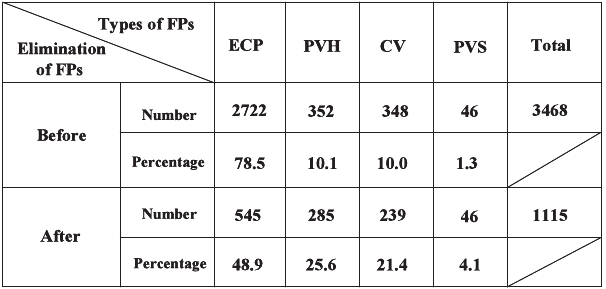
\includegraphics[width=0.8\textwidth]{Images/5_yokoyama2007testing.png}
%	\caption{Elimination of false-positives. Perivascular spaces (\textsc{pvs}) see no reduction. They make only 4.1\% of false-positives under the definition in \cite{Yokoyama2007}.}
%	\small Image taken from \cite{Yokoyama2007}
%	\label{litrev-yokoyama-fps}
%\end{figure}
%
%Yokoyama et al. suggest that further reductions in false-positives could be attained through the use of FLAIR imaging. Lacunes are found to have a low intensity in T1-weighted imaging and a high intensity in T2-weighted imaging. In FLAIR imaging, lacunes are also found to have a low intensity, but not as low as the surrounding CSF, and often have a hyperintense rim \cite{WardlawJ.M.2013Nsfr}. 
%
%Further improvements could be made by using multiple slices for each candidate, increasing image context. Using 3D information, the axial slices above and below a candidate could be used to further eliminate false-positives. This is particularly relevant when a candidate lacune appears on only a single axial slice, or when the candidate diverges from the indicative ovoid shape in surrounding slices. Including this information would assist in differentiation between lacunes and perivascular spaces, since perivascular spaces can appear rectangular along the coronial or saggital plane.
%
%\subsection*{Concerns}
%
%Although the testing sensitivity was high, it was not high enough for the model to be usable on its own. Model improvement is required before it can be used to aid clinicians reliably.
%
%Yokoyama et al. made the assumption that lacunes only occur deep within the brain, within and surrounding the basal ganglia. This was the motivation behind extracting data around the cerebral ventricle. However, this assumption is not always satisfied. Though less common, lacunes have been found in other brain regions, including the cerebrum.
%
%The feature definitions used for the model also make it difficult to identify perivascular spaces. In this model, perivascular spaces were defined as small, circular regions of diameter less than 3 mm, located at the lower basal ganglia. This specification meant that the model was not sensitive to enlarged perivascular spaces, which can have a diameter up to 10 mm and can occur anywhere in the grey and white matter of the brain \cite{WardlawJ.M.2013Nsfr}. This change in definition contributes to the seemingly low false-positive presence that PVS exhibit in the data.
%
%It should be mentioned that this model is dependent on a number of existing architectures. The first is the identification and extraction of particular brain regions. In this model, Yokoyama et al. were able to use existing binarisation techniques to extract the cerebral ventricle. Each sample also requires a calculated area, circularity and gravitational centre. Each of these calculations requires sufficient time and resources, particularly if these calculations are to be conducted manually.
%
%Finally, the proportion of false-positives is still relatively high. The sensitivity after the second phase is 90\%, which is substantial but still not accurate enough to warrant full automation of the process. Of particular concern is the proportion of perivascular spaces falsely marked as lacunes. Though they appear similar to lacunes, perivascular spaces do present some slight shape and intensity differences.

%In 2012, Wang et al. \cite{WangY.2012Msow} developed an algorithm that labels three features: \textsc{wmh}, lacunes in the cerebral cortex (cortical infarcts), and lacunes beneath the cerebral cortex (lacunar infarcts). The model was provided with 272 scans, each capturing T1-weighted, T2-weighted and \textsc{flair} images. In the first stage of the algorithm, the T1-weighted images are used to segment the brain into white matter, grey matter and \textsc{csf}. Average intensities are calculated for each segmented region and for each image type. Candidate features are identified based on their intensity relative to these these averages. The resulting sensitivity rate for lacunes is 80.6\% and 006 false-positives per slice.

\section{Machine learning}\label{litrev-ml}

This section describes a number of models that were developed using machine learning techniques. The model by Yokoyama et al. \cite{Yokoyama2007} suffered from a lower sensitivity rate, possibly caused by lack of information extracted from the images. Machine learning techniques seek to identify features that are not always easily interpreted, but have had promising results. 

The first attempts were made by Uchiyama et al. in 2007 \cite{Uchiyama20071554, Uchiyama2007b} as a continuation of the model by Yokoyama et al. \cite{Yokoyama2007}. The data consisted of 132 scans totalling 1143 images of T1 and T2 weighting. Once candidates have been identified, the models undergo false-positive reduction. Twelve location based features are identified: x and y coordinates, intensity differences in T1 and T2, four nodule shape variables, and four combined nodule and linear shape variables.

These features were input into two different machine learning algorithms: a support vector machine (machine learning algorithm for discrimination tasks) and a neural network. The support vector machine resulted in a sensitivity of 96.8\%, with 0.76 false-positives per slice. The second model was a neural network, with a sensitivity of 96.8\% and 0.30 false-positives per slice.

In 2015, Uchiyama et al. \cite{Uchiyama2015} augmented their previous models by matching candidates with a number of lacune templates. To improve the efficiency of the matching process, data was reduced to a lower dimensional space through principal component analysis. False-positives were reduced by 34.1\%, with the final model having a sensitivity of 96.8\% and 0.47 false-positives per slice.

The substantial rise in sensitivity in comparison to the original model \cite{Yokoyama2007} confirms that additional information was required to improve lacune detection. However the included variables remain location dependent and require either existing algorithms or significant time resources during data collection.


%\section{Yokoyama 2007}
%
%Lacunar infarct regions are classified into two types: isolated regions and regions next to hyperintensities. Isolated lacune candidates are found using multiple-phase binarisation. Candidates next to hyperintense structures are detected by pre-processing and subtracting images. Candidate regions are generated based on area, circularity and gravitational centre. False-positives are first reduced by removing candidates at the edge of the image. Next compare the candidates against mean pixel values of surrounding circular regions.
%20 lacune samples were used to adjust area, circularity and gravitational centre thresholds. 673 images used for testing. Sensitivity 90.1\%, specificity 30.0\%, 1.7 false-positives per slice.
%
%\section{Uchiyama 2007a}
%
%Data consists of 1143 of T1 and T2 weighted images each, from 132 scans. The search region was restricted (to what?). Initial candidates found by using top-hat transforms and multiple-phase binarisation to T2 weighted images. False-positives eliminated by determining 12 features: x and y coordinates, intensity differences in T1 and T2, and by extracting 4 scales of nodular component images, and 4 scales of nodular and linear component images.
%
%In this first model type, the 12 features were processed through a support vector machine. This resulted in a sensitivity of 96.8\%, with 0.76 false-positives per slice.
%
%\section{Uchiyama 2007b}
%
%This model was identical to the first (Uchiyama 2007a), with the difference that the 12 features were passed through a neural network instead of a support vector machine. This resulted in a sensitivity of 96.8\%, with 0.30 false-positives per slice.
%
%\section{Uchiyama 2008}
%
%Developed CAD scheme for classification of lacunes and perivascular spaces. 109 MRI scans of T1 and T2-weighted images. 89 lacune images and 20 enlarged perivascular spaces. White top-hat transform to enhance T2 images. Grey-level thresholding to segment lesions. Determine the size, shape, location, and T1 and T2 intensities. These features were input into a neural network to distinguish between lacunes and perivascular spaces. Area under ROC curve (true positive/false-positive ratio - only good for discriminant analysis) of 0.945.
%
%\section{Uchiyama 2015}
%
%Improvement on their previous model (96.8\% sensitivity and 0.71 false-positives per slice), by template matching in the eigenspace. However, large number of templates needed, and cross-correlation is time consuming. To resolve these issues, template matching was used in a lower dimensional space via principal component analysis. Dataset consisted of 1143 images of T1 and T2, from 132 patients (same dataset as 2007 studies?). 34.1\% of false-positives eliminated from previous attempt. Final performance was 96.8\% sensitivity, 0.47 false-positives per slice.
%
%\section{Wang 2012}
%
%Wang et al. label all three: \textsc{wmh}, cortical infarcts and lacunar infarcts. They first segment the brain tissues into white matter, grey matter and CSF using the T1-weighted scans. Hyperintense structures identified using FLAIR images. The three features are labelled based on all three weighted images, T1, T2 and FLAIR. 


%Wang et al. (2012) detect lacunes by dilating the white matter mask and using a rule-based pruning of false-positives considering their intensity levels compared to the surrounding white matter tissue.
%

%\section{Uchiyama2007a - support vector machines}

%In 2007, Uchiyama et al. \cite{Uchiyama20071554} used a machine learning algorithm to develop a computer-assisted diagnosis (CAD) program for lacune identification. In particular, false-positive reduction took the form of a support vector machine (SVM).
%
%Their data consisted of 132 MRI scans, each with T1-weighted and T2-weighted images, giving a total of 1143 axial slices in the dataset. 
%
%Similar to the method conducted by Yokoyama et al. \cite{Yokoyama2007}, Uchiyama et al. identified candidate lacunes of two forms: isolated lacunes, and those close to the cerebral ventricle. Isolated lacunes were determined by establishing a threshold, as these points exhibit a higher intensity compared to the surrounding tissue. For lacunes close to the cerebral ventricle, their higher intensity can be masked by the intensity of the surrounding ventricle. To address this, Uchiyama et al. used top-hat transforms on the T2-weighted images, a method that is specialised for extracting small details from image data.
%
%% Candidate lacune identification
%\begin{figure}[ht]
%	\centering
%	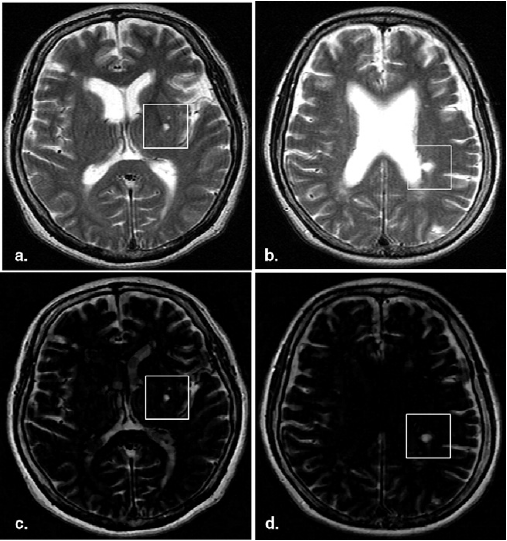
\includegraphics[width=0.8\textwidth]{Images/5_uchiyama_candidates.png}
%	\caption{Candidate lacune detection. Isolated lacune in a), with resulting top-hat transform shown in c). Lacune in b) is next to the cerebral ventricle, with top-hat transform shown in d).}
%	\small Image taken from \cite{Uchiyama20071554}
%\end{figure}
%
%false-positives were reduced using support vector machines. 12 features were used in false-positive reduction, including the candidate's x and y location, signal differences in the T1-weighted and T2-weighted images, and filtered images based on 4 nodular components and 4 combined nodular and linear components. This model produced a sensitivity of 96.8\%, with 0.76 false-positives per slice.
%
%\subsection*{Concerns}
%
%Model sensitivity is high enough to warrant usage of the model, though not high enough for full dependency. As described by Uchiyama et al., the model was designed as a CAD scheme, to run alongside manual rating by clinicians. The model still requires a user to oversee and confirm its results. 
% 
%Similar to the model developed by Yokoyama et al. \cite{Yokoyama2007}, the model developed by Uchiyama et al. was not able to distinguish between lacunes and enlarged perivascular spaces. Despite the data containing analysis on the nodular and linear nature of the candidate, the model was unable to make this distinction. Therefore, users of the CAD system must take care to confirm that the suggested candidates are not enlarged perivascular spaces.
%
%Many of the variables included in the method are dependent on other existing techniques. For instance, Uchiyama et al. explain that the nodular and linear components were determined via a newly explored filter bank technique. This technique was not well described, and as such, the model may be difficult to recreate.
%
%Another issue is the coordinate system. The model uses the x and y coordinates of the candidate to reduce false-positives. The coordinates themselves do not have any innate information about the structure of the brain. It is possible for the same x and y values to link to differing regions across brain scans. It is not certain that particular coordinates will align with a brain structure that has a significant influence on the presence of lacunes. This is especially the case for candidates deep in the brain, as many brain structures sit close together. 
%
%Under the assumption that the x and y coordinates are indicative of lacune probability, the usage of location data may still incorrectly influence outcomes. Lacunes can be found throughout the brain, including in the cerebrum. 
%
%\section{Neural Networks}
%
%Uchiyama et al. \cite{Uchiyama2007b} improve their previous model \cite{Uchiyama20071554} by altering the method used for reducing false-positives. The support vector machine was swapped with a neural network, using the same 12 input features.
%
%The sensitivity of the model to lacunar infarcts remains the same, at 96.8\%. The number of false-positives drops to 0.30 false-positives per slice.


\section{Convolutional neural networks}\label{litrev-cnn}

We will now discuss the convolutional neural network structure utilised by Ghafoorian et al. \cite{GhafoorianM.2017Dml3}. This model forms the basis of our adjusted location-independent model. This model consists of two phases; candidate generation using a \textsc{cnn}, and false-positive reduction using a 3D \textsc{cnn} and candidate location data.

\subsection*{Candidate Detection}

The data set consists of 1075 \textsc{mri} scans split into training, validation and testing sets of size 868, 96 and 111 respectively. Each scan contains two image weightings: T1-weighted and \textsc{flair}. Data samples are generated by randomly sampling axial slices of dimension 51$\times$51 pixels, each called a \textit{patch}. The model is trained to detect lacunes at the centre of each patch, returning either a positive response $(1, 0)^\intercal$ or negative response $(0, 1)^\intercal$. Combining the T1-weighted image, \textsc{flair} and response gives samples containing two 51$\times$51 pixel images and a response vector in $\mathbb{R}^2$. For use in convolution, the T1-weighted image and the \textsc{flair} image are treated as separate colour channels. Samples were generated such that there were twice as many negative samples as positive, totalling $3.2\times10^5$ training samples.

% Candidate model structure
\begin{figure}[ht]
	\centering
	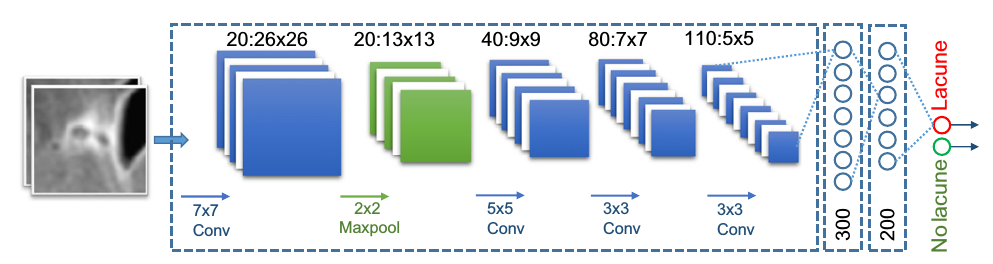
\includegraphics[width=\textwidth]{Images/5_ghafoorian_model1.png}
	\caption{Candidate detection model structure.}
	\small Image taken from \cite{GhafoorianM.2017Dml3}
	\label{litrev-ghafoorian_model1fig}
\end{figure}

The \textsc{cnn} is made of seven layers, as shown in Figure \ref{litrev-ghafoorian_model1fig}. The first four are convolutional layers, followed by three fully connected layers. The four convolutional layers contain 20, 40, 80 and 110 filters, with filter sizes 7$\times$7, 5$\times$5, 3$\times$3 and 3$\times$3 respectively. A max pooling layer is included between the first and second convolutional layer, with a filter size of 2$\times$2 and stride of 2. No zero padding is applied to the convolution or pooling layers. The convolution is followed by three fully connected layers of 300, 200 and 2 neurons.

Batch normalisation and ReLU activation is applied to all neurons. Dropout is applied to the fully connected layers, with a rate of 0.3. All weights are intialised using the He method \cite{HeKaiming2015DDiR}. Training is conducted by stochastic gradient descent with the Adam optimiser. Each training batch has a sample size of 128. A decaying learning rate is used, from $5\times10^{-4}$ to $10^{-6}$ by the last epoch.

Cross-entropy loss is used to assess the model at the end of each batch. L2-regularisation is used, with the penalty term set to $10^{-4}$. The final layer applies softmax activation to ensure the output follows a probability distribution. An early stopping algorithm is used such that the model with the highest validation accuracy is saved.

Ghafoorian et al. comment that the model can be computationally intensive to run on many data points. To improve speed, the fully connected layers are converted into convolutional layers.

Candidate lacunes are identified by feeding 51$\times$51 samples of the tested scan through the trained \textsc{cnn}. For each given sample, the model outputs a lacune classification probability. Once this has been completed for the whole volume, a 10$\times$10 sliding window identifies local maximums in the resulting probabilities. Sliding window samples with lacune probabilities below 0.1 are removed and the remaining samples are lacune candidates to be input into the second phase of the model. Note that there were no performance diagnostics provided for the first model stage.

%
%Entire model is made up of two neural networks.
%
%The first is trained such that it detects candidate lacunes.
%
%The second then takes the candidate lacunes, and processes them through a more thorough 3D CNN to finalise the outcome.
%
%\subsection{First Phase - Candidate Detection}
%
%Takes in 51x51 samples, where the T1 and FLAIR components are treated as separate channels. Twice as many negative samples as positive, with a total of 320K for training.
%
%Seven layer CNN:
%- 4 convolutional, with 20, 40, 80, 110 filters, with size 7x7, 5x5, 3x3, 3x3 respectively.
%- 1 pooling layer: size 2x2, stride 2, after first conv layer
%- 3 fully connected layers: sizes 300, 200 and 2
%- Softmax output layer
%
%All neurons went under batch normalisation.
%
%Weights initialised by the He method.
%
%ReLU activation to prevent vanishing gradient problem
%
%Dropout of 0.3 on fully connected layers
%
%Training conducted by stochastic gradient descent, Adam optimiser. Learning rate decayed, from 5e-4 to 1e-6
%
%Batch size of 128
%
%Categorical cross-entropy loss, with L2-regularisation (Ridge regression), lambda2 = 0.0001
%
%Early stopping - model with highest accuracy on validation set
%
%
%This method can be slow on its own. Translate the fully connected layers to convolutional layers, via shift-and-stitch method.
%
%Local maxima extraction (10x10 window) - picking those with likelihood lower than 0.1.
%
%
%Didn't mention: number of epochs to train. How pooling and convolutions were padded. Diagram implied no padding, but diagram dimensions weren't correct. 

\subsection*{False-positive reduction}

The second phase of the model serves to reduce the number of false-positives returned by the first stage of the model. This model uses a 3D \textsc{cnn}, adding additional contextual information to the image. Each data point is captured at three different resolutions, 32$\times$32$\times$5, 64$\times$64$\times$5 and 128$\times$128$\times$5, to capture varying levels of contextual information. These samples are reduced to dimension 32$\times$32$\times$5 before input into the model to lower the number of variables. In total, there were $3.85\times10^5$ samples for training, and $3.5\times10^4$ for validation. 

Each resolution is fed through its own 3D \textsc{cnn}, as shown in Figure \ref{litrev-ghafoorian_model2fig}. Each \textsc{cnn} branch contains six convolutional layers and a fully connected layer. The convolutional layers have 64, 64, 128, 128, 256 and 256 filters of sizes 3$\times$3$\times$2, 3$\times$3$\times$2, 3$\times$3$\times$1, 3$\times$3$\times$1, 3$\times$3$\times$1 and 3$\times$3$\times$1 respectively.

% False-positive reduction model structure
\begin{figure}[ht]
	\centering
	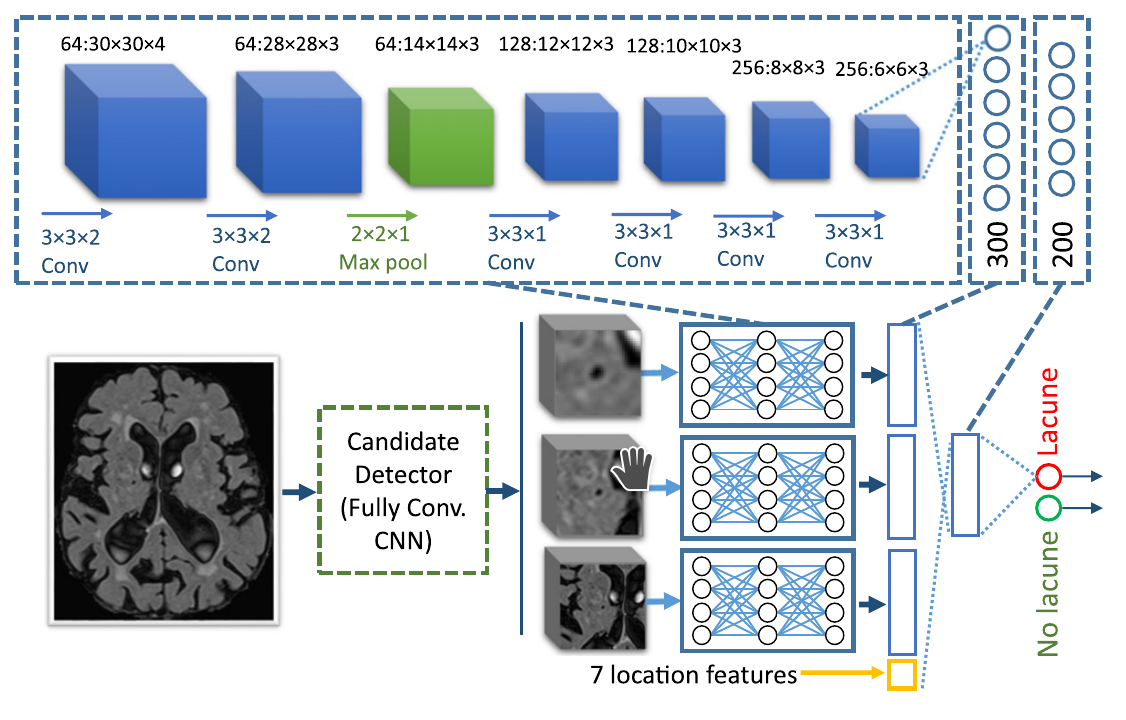
\includegraphics[width=\textwidth]{Images/5_ghafoorian_model2.png}
	\caption{False-positive reduction model structure.}
	\small Image taken from \cite{GhafoorianM.2017Dml3}
	\label{litrev-ghafoorian_model2fig}
\end{figure}

A single max pooling layer is placed after the second convolution layer, of size $2\times2\times1$. In each resolution branch, the final convolution layer is followed by a fully connected layer of 300 neurons. The $3\times300$ fully connected neurons are concatenated together with seven additional location variables. For each candidate, these location features include the $x$,$y$ and $z$ coordinates, and distances to the left and right ventricles, cortex, and midsagittal brain surface.

The 907 fully connected neurons are passed to two final fully connected layers of size 200 and 2 neurons. The final layer consists of a softmax activation to output the lacune probabilities. All weights are He initialised. All neurons, excepting the output layer, have ReLU activation and are batch normalised. The fully connected layers have a dropout rate of 0.5. 

The cost function chosen was cross-entropy with L2-regularisation and penalty parameter $2\times10^{-15}$. This was minimised using stochastic gradient descent with an Adam optimiser. The learning rate is initialised as $5\times10^{-4}$. If training accuracy drops, the learning rate decays by a factor of 2. Each training batch contained 128 samples.

The model was trained for 40 epochs, with the final model chosen to maximise validation accuracy. A number of hyper-parameters were chosen by maximising validation accuracy. These included network depth, batch size, the initial learning rate and decay factor, penalty parameter, and dropout rate. The resulting model exhibited a sensitivity of 97.4\% and an average of 0.13 false-positives per slice.




%
%\subsection{Second Phase - false-positive Reduction}
%
%This model uses data at different scales around each candidate lacune. 
%
%Input data of each point at three different scales: 32x32x5, 64x64x5, 128x128x5.
%
%Each of these scales is reduced to 32x32x5, then put through a separate branch of the network.
%
%385K training, 35K validation.
%
%Three separate branches of convNets, one for each scale. Each branch contains:
% - 6 conv layers (64, 64, 128, 128, 256,256 filters, with sizes 3x3x2, 3x3x2, 3x3x1, 3x3x1, 3x3x1, 3x3x1)
% - 1 pooling, size 2x2x1, placed after second conv layer
% - Fully connected layer of 300 neurons
% 
% The 3x300 fully connected neurons were concatenated with 7 addition location feature inputs.
% 
% These location features include:
%  - x,y,z coordinates
%  - distances from left ventricle, right ventricle, cortex and midsaggital brain surface.
%
%Then the 907 neurons are fully connected to two more fully connected layers, of size 200 and 2 neurons. 
%These are fed through a softmax classifier to output the final result.
%
%All weights are He initialised 
%
%All activations are ReLU, and are batch normalised.
%
%Fully connected layers have a dropout of 0.5.
%
%Cost function is cross entropy with L2 regularisation, lambda2 = 2e-5. 
%
%Stochastic gradient descent, Adam optimiser. Decaying learning rate, from 5e-4, decay factor of 2 when training accuracy dropped. 
%
%Training for 40 epochs, batch size of 128.
%
%Chose model with highest validation accuracy. 
%
%Hyper-parameters were also chosen such as to attain highest validation accuracy. These hyper-parameters included network depth, batch size, initial learning rate, learning decay factor, lambda2 and dropout rate. This is done during the validation stage. Make several models, with differing hyper-parameters, with performance compared using the validation set. Then whichever model performs best on this validation set is chosen, and final performance judged by the test set.
%
%Data was augmented during test time: cropping and flipping. Predictions of the 242 variants per sample were averaged.
%
%Didn't mention: stride of pooling. Assumed 2 from diagram.
% 
%\subsection{Model performance}

\section{Proposed changes}\label{litrev-changes}

The models trained by Uchiyama et. al. \cite{UchiyamaYoshikazu2007Ioad}, Yokoyama et. al. \cite{Yokoyama2007} and Ghafoorian et al. \cite{GhafoorianM.2017Dml3} rely on location variables generated for each candidate lacune. Ghafoorian et al. claimed that the inclusion of location variables helps to differentiate lacunes from perivascular spaces, which occur primarily in the basal ganglia. However, lacunes can occur throughout the brain white and grey matter \cite{WardlawJm2013Mosc} and so adding these location variables could result in incorrect classification should lacunes occur in less frequently observed regions.

The inclusion of location data requires extra data pre-processing. These variables are calculated in relation to other located brain structures, however these locations are not inherently included within \textsc{mri} scan data. Instead these variables are generated prior to model usage and require either visual estimation or a feature extraction algorithm \cite{Uchiyama2007b, UchiyamaYoshikazu2007Ioad}. If the variables are to be determined visually, the variables for each candidate lacune have to be determined separately and this would require significant extra data preparation time. If location variable extraction algorithms exist, as in the model by Uchiyama et al. \cite{UchiyamaYoshikazu2007Ioad}, additional measurement errors could also make location-based inference inaccurate.

In this study, we attempt to simplify and adapt the model by Ghafoorian et al. \cite{GhafoorianM.2017Dml3} to the available data set (see Section \ref{data}). A key component of the existing model is the removal of false-positives by analysing the three-dimensional context and location-based variables. These variables include the $x$, $y$ and $z$ coordinates, and distances between the candidate and the ventricles, cortex and midsagittal plane. Without the architecture to determine these distances, these variables have to be determined manually. In addition, the  $x$, $y$ and $z$ coordinates are not standardised between scans. Consequently, the coordinates across images do not necessarily align with the same brain structures.

The available image pre-processing pipeline (see Section \ref{data}) allows for the automated extraction of brain tissue. This may reduce the complexity of the task such that location-based variables may not be required. We therefore simplify and assess the existing model when performed on brain tissue extracted data, independent of location-based variables.


%- All previous models have made some use of location data. In particular, Ghafoorian used x/y/z, and distances from the candidate to particular brain structures. However, lacunes can appear in other regions of the brain, including regions far from the basal ganglia. The location data requires the location of the ventricles, cortex and midsaggital plane. To do this in an automated fashion requires an algorithm that can find these brain features. This requires additional estimation. Try to develop an algorithm that is independent of location data. Rely more on the image.
%
%- Instead of trimming candidates in a second phase, try to determine strong candidates from just the first phase to create an accurate CAD program. Then clinicians can be presented with candidate lacunes, and still conduct false-positive reduction themselves
%


%
%\section{Convolutional Neural Networks}
% 
%Ghafoorian et al. \cite{GhafoorianM.2017Dml3} utilised the fully convolutional nature of the initial detection model. This allows for fast image processing in comparison to fully connected layers, for 3D volumes. In addition, Ghafoorian et al. additionally utilised a multi-resolution convolutional neural network, along with 7 additional location features for false-positive reduction.
%
%\section{xgboost}
%

 


%%%%%%%%%%%%%%%%%%%%%%%%%%%%%%%%%%%%%%%%%%%%%%%%%%%%%%%%%%%%%%%%%%%%%%%%%%

%\clearpage

\addcontentsline{toc}{chapter}{References}

\bibliographystyle{apalike}
\bibliography{bibliography.bib}

%\bibliographystyle{apacite}
%\bibliography{mybib.bib}

